\section{Design}
\subsection{TCP/IP}
%1 pourquoi utiliser xml, tcp, ip ... consomme de la batterie + UDP pas fiable ?
\begin{frame}
 \frametitle{Design et implications}
 TCP/IP à la place des données brutes:\\
 \vspace{5mm}
 \textbf{$\rightarrow$} Accès à de nombreux outils\\
 \textbf{$\rightarrow$} Plus de chances d'être accepté par la communauté.\\
 \vspace{5mm}
\begin{block}{Inconvénient}
Overhead imposé par les standards, techniques de réduction de taille des paquets nécessaires
\end{block}
 
\end{frame}
%utiliser une encapsulation tcp/ip augmente fortement la taille du message (40 octets) + inserer tableau
\begin{frame}
\frametitle{TCP/IP overhead}
Augmentation de la taille des paquets : header de 40 octets.\\
\vspace{5mm}
Exemple de transfert de 10 octets bruts avec et sans TCP/IP: \\
\begin{center}
\begin{tabular}{|c|c|c|c|}
\hline
~ & Minimum & Avec TCP/IP & TCP/IP\\
~ & requis & ~ & overhead\\
\hline
Paquets & 2 & 8 & 300\% \\
Octets & 11 & 338 & 2793\% \\
Délai (ms) & 6 & 375 & 6150\% \\
\hline
\end{tabular}
\end{center}
\end{frame}

\begin{frame}{Améliorations des performances}
\begin{itemize}
\item Connexion TCP persistante : suppression des handshakes à chaque transmission
\item Désactivation du \textit{Delayed ACK} : gain de temps du à la taille des messages envoyés
\item Réduction du timeout de retransmission : paquets perdus réenvoyés plus vite
\item Sleep mode entre messages TCP : radio éteinte durant les délais minimaux
\end{itemize}
\end{frame}

%inserer figure 3
\begin{frame}{Désactivation du \textit{Delayed ACK} }
\begin{figure}
  \begin{minipage}[c]{.46\linewidth}
  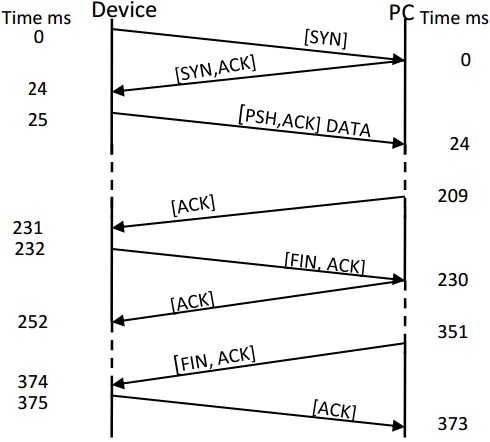
\includegraphics[scale=0.4]{figures/TCPlatences.jpg}
  \caption{TCP}
  \label{tcplatences}
 \end{minipage}
 \begin{minipage}[c]{.46\linewidth}
  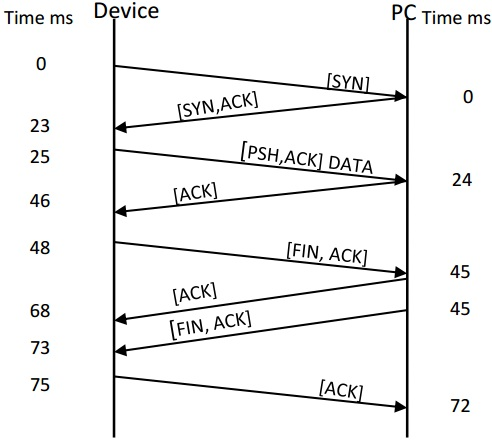
\includegraphics[scale=0.4]{figures/delayedACK.jpg}
  \caption{Delayed ACK désactivé}
  \end{minipage}
 \end{figure}
\end{frame}
%TCP persistante

%retransmission pas bien + figure + on diminue fortement le timeout pour éteindre la radio le plus vite possible
\begin{frame}
 \frametitle{Retransmission}
 \begin{figure}
  
  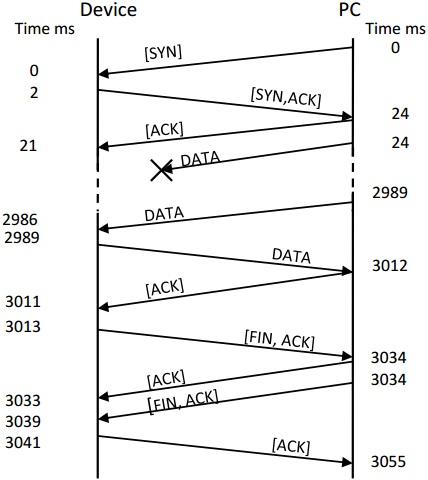
\includegraphics[scale=0.5]{figures/TCPretransmission.jpg}
  \caption{Retransmission}
  \label{retransmission}
  
 \end{figure}
\end{frame}
%radio off entre les messages + valeur du temps minimum de dodo

\subsection{service web}
% duty cycle, il ne doit avoir transmission de message que lors de l'évenement.
\begin{frame}{Duty cycle}
 \framesubtitle{WS-eventing}
 La majorité des capteurs n'ont besoin de transférer des messages que lors d'un événement. Grâce au WS-eventing, le capteur peut entrer en sleep mode entre les événements.\\
 \vspace{3mm}
 Le WS-eventing est composé de 5 entités fonctionnelles :
 \begin{enumerate}
  \item \textit{Event source} %génère une interruption (détecteur de fumée)
  \item \textit{Event subscribers} %sont Veulent être informé de l'événement.
  \item \textit{Subscription manager} %accepte et gère les demandes d'inscriptions.
  \item \textit{Event subscription database} %stocke les inscriptions actives.
  \item \textit{Notification manager} %retransmet l'interruption à tous les intéressés enregistrés dans la base de donnée.
 \end{enumerate}
 %c'est comme le design patern observer
\end{frame}

\begin{frame}
 \frametitle{WS-eventing}
 \framesubtitle{Architecture}
 \begin{figure}
  \centering
  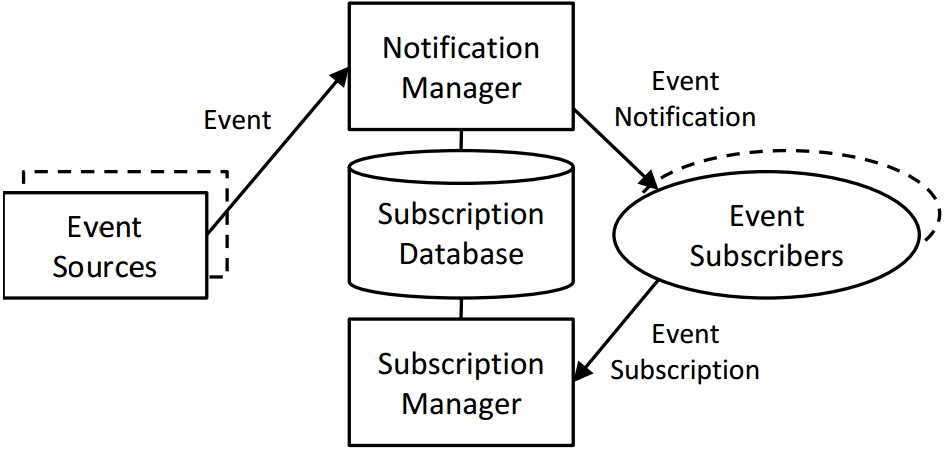
\includegraphics[scale=0.43]{figures/eventing.jpg}
  \caption{Architecture Web services eventing}
 \end{figure}
 %Implémenté dans le contrôleur.
\end{frame}
%utilisation de fichier wsdl + expliquer ce que c'est + les protocoles disponible, on chois http
\begin{frame}
 \frametitle{WSDL}
 Fichier WSDL : décrit les méthodes disponibles sur le capteur.\\ %(développé dans la section Prototypage).
 3 protocoles supportés pour les requêtes: SOAP, HTTP et MIME.\\
 \vspace{3mm}
 \begin{center}
 \begin{tabular}{|c|c|c|c|}
 \hline
 Nom de la méthode & SOAP 1.1 & SOAP 1.2 & HTTP\\
 \hline
 GetTemperature & 491 & 442 & 162\\
 GetTemperatureResponse & 479 & 499 & 258\\
 SetTemperature(70) & 528 & 482 & 202\\
 SetTemperatureResponse & 455 & 475 & 230\\
 \hline
 \end{tabular}
 \end{center}
 $\Rightarrow$ protocole HTTP pour les requêtes.
\end{frame}
\subsection{XML}
%utilisation de xml. + tableau + expliquer chaque ligne du tableau.
\begin{frame}
 \frametitle{Optimisation du message XML}
 La requête et la réponse peut aussi être encodé dans un XML en utilisant HTTP POST.
 Puisque les informations présentes dans le messages seront toujours une liste de noms de méthodes, leurs arguments et leurs valeurs décrit dans le WSDL, il suffira juste d'un algorithme de parsing pour le lire.
 Ce qui réduit la place en mémoire et la complexité.\\
 \vspace{4mm}
 Ensuite, il existe plusieurs astuces pour réduire la taille du message.\\
 \begin{center}
  \begin{tabular}{|c|c|c|c|c|}
   \hline
   Compression & Get & Get & Set & Set\\
   ~ & Temp & TempResponse & Temp & TempResponse\\
   \hline
   Original & 85 & 181 & 125 & 153\\
   \hline
   Xmlppm & 65 & 98 & 85 & 92\\
   Zip & 114 & 157 & 138 & 151\\
   \hline
   Comp1 & 81 & 101 & 101 & 107\\
   Comp2 & 26 & 46 & 46 & 53\\
   \hline
  \end{tabular}
 \end{center}
\end{frame}

\begin{frame}
 \frametitle{Optimisation du message XML}
 \framesubtitle{Techniques}
 \begin{itemize}
  \item \textbf{Original}, le message XML Initial.
  \item \textbf{Zip}, une méthode de compression.
  \item \textbf{Xmlppm}, une méthode de compression spécifique aux fichier XML.
  \item \textbf{Comp1}: On remplace les tags par une valeur codée en 1 octet.
  Un dictionnaire Nom de méthode $\rightarrow$ valeur est fourni par le capteur et devra être utilisé coté utilisateur (plutot coté controleur).
  %Le dictionnaire sera demandé typique qu'une fois.
  \item \textbf{Comp2}: Le header (<?xml version=...) et le namespace URL sont remplacés par des tags compacts.
 \end{itemize}
\end{frame}
